\documentclass[12pt]{article}

\usepackage{sbc-template}
\usepackage{graphicx,url}
\usepackage[utf8]{inputenc}
\usepackage[brazil]{babel}
\usepackage{lipsum}
%\usepackage[latin1]{inputenc}  
\usepackage{amsmath}
\usepackage[portuguese,ruled,vlined]{algorithm2e}
%\usepackage[portuguese,ruled,vlined,linesnumbered]{algorithm2e}
\usepackage{blindtext}
\usepackage{xcolor}
\usepackage{caption}
\usepackage{subcaption}
\usepackage{colortbl}
\usepackage{adjustbox}
\usepackage{tikz}
\usepackage{pgf}
\usepackage{multirow}
\usepackage{pgfplots}
\usepackage{amsmath}
\usepackage{float}
     
\sloppy

\title{Componentes Conexos em Processador Multicore}
\author{Patreze A. Chita \inst{1}, Nahri. B. Moreano\inst{1}}
\address{Faculdade de Computação -- Universidade Federal do Mato Grosso do Sul (UFMS) \\ Caixa Postal 549 -- 79.070.900 -- Campo Grande -- MS -- Brazil
\email{patrezechita@gmail.com, nahri@facom.ufms.br}
}

\begin{document} 

\maketitle
     
\begin{resumo} 
Este artigo apresenta dois algoritmos para solucionar o problema dos componentes conexos de um grafo não orientado. Foram implementadas uma solução sequencial conhecida da literatura e uma solução paralela baseada em uma descrição de alto nível, também da literatura. É apresentado os detalhes dessa implementação paralela e discutida uma análise sobre o desempenho dos dois algoritmos.
\end{resumo}

\section{Introdução}
Seja um grafo G=(V, E) não orientado, G é conexo se, para qualquer par \{v, u\} de vértices $\in$ V, existe um caminho com extremos v e u. Um componente conexo de um grafo G é qualquer subgrafo conexo maximal de G. Sendo assim, cada vértice de um grafo G pertence a um único componente.

Encontrar os componentes conexos de um grafo é o coração de muitas das aplicações com grafos. Por exemplo, considere o problema de identificar grupos em um conjunto de itens. Podemos representar cada item por um vértice e adicionar uma aresta entre par de itens que são considerados semelhantes. Os componentes conexos desse grafo correspondem a diferentes classes de itens~\cite{Skiena:2008}.

O objetivo deste trabalho é implementar e analisar duas soluções para o problema dos componentes conexos, sendo uma sequencial e outra paralela, ambas da literatura. Analisando o desempenho obtido pelos algoritmos, poderemos concluir se a paralelização do problema de fato produz algum ganho em relação ao algoritmo sequencial.

No capítulo 2 são apresentados os dois algoritmos, sendo o sequencial integralmente e o paralelo somente a descrição da literatura. No capítulo 3 é apresentada a implementação do algoritmo paralelo. No capítulo 4 é feita uma análise sobre o desempenho obtido pelos dois algoritmos e como foi feita essa medição. No capítulo 5 é apresentada a conclusão deste trabalho.

\section{Algoritmos Sequencial e Paralelo para Componentes Conexos}
O algoritmo sequencial apresentado neste trabalho é baseado na busca em profundidade (\emph{depth-first search}, DFS). Assim como a busca em profundidade, outros algoritmos sequenciais podem ser utilizados para resolver o problema dos componentes conexos, sendo um deles, o algoritmo baseado nas operações \emph{Union-Find}. Tanto o algoritmo da busca em profundidade quanto o baseado nas operações \emph{Union-Find} são descritos em~\cite{Sedgewick:2011}. Em~\cite{Grama:2003} também é apresentado o algoritmo de busca em profundidade para solucionar sequencialmente o problema dos componentes conexos, assim como, é apresentado de maneira alto nível uma possível paralelização deste algoritmo.

\subsection{Algoritmo Sequencial Baseado em Busca em Profundidade}

Inicialmente, uma maneira natural de se resolver o problema dos componentes conexos é executando uma busca em profundidade em um determinado grafo. O resultado disso é uma floresta composta por várias árvores, que são por definição, conexas e acíclicas. Portanto, um algoritmo de busca em profundidade levemente modificado pode resolver sequencialmente o problema dos componentes conexos. Essa afirmação é corroborada por~\cite{Grama:2003} e~\cite{Sedgewick:2011}.

Como resultado de uma busca em profundidade, todo vértice que pertence a uma mesma árvore, está em um mesmo componente do grafo. Nota-se que isso é verdade, pois, partindo de um vértice, será acessado outro que compartilha uma aresta, portanto, existe um caminho entre esses dois vértices. A modificação necessária no algoritmo de busca em profundidade é que, toda vez que um vértice é ``visto'' pela busca, todos os próximos vértices (acessados a partir dele) estarão no mesmo componente conexo. O Algoritmo~\ref{alg_seq} demonstra o funcionamento sequencial implementado da busca em profundidade, com a modificação para se armazenar a informação de qual componente pertence cada vértice.

\begin{algorithm}[H]
    \DontPrintSemicolon
    \SetArgSty{textnormal}
    \caption{Algoritmo sequencial para componentes conexos}
    \label{alg_seq}
    \SetKwProg{ComponentesConexos}{ComponentesConexos}{}{}
    \ComponentesConexos{{\normalfont(grafo G = (V, E))}}
	{
        nComponentes $\gets$ 0\;
        \ParaCada{vértice v $\in$ V}
        {
            visitado[v] $\gets$ FALSO\;
        }
        \ParaCada{vértice v $\in$ V}
        {
            \Se{visitado[v] = FALSO}
            {
                \textbf{DFS}(v)\;
                nComponentes $\gets$ nComponentes + 1\;
            }
        }
    }
    \SetKwProg{DFS}{DFS}{}{}
    \DFS{{\normalfont(vértice v)}}
    {
        componente[v] $\gets$ nComponentes\; 
        visitado[v] $\gets$ VERDADEIRO\;
        \ParaCada{vértice u $\in$ Adj[v]}
        {
            \Se{visitado[u] = FALSO}
            {
                \textbf{DFS}(u)\;
            }
        }
    }
\end{algorithm}

\subsection{Algoritmo Paralelo Baseado em Busca em Profundidade e nas Operações Union/Find}

Em~\cite{Grama:2003}, uma descrição de como paralelizar esse processo sequencial da busca em profundidade é apresentada. Sua sugestão, mesmo sendo bem alto nível, é suficiente para entender o funcionamento do algoritmo paralelo e nos dá os passos necessários para a implementação do algoritmo. 

Primeiramente, deve-se dividir a matriz de adjacências do grafo por todos os processadores, assim sendo, cada processador vai receber um ``pedaço'' do grafo, no qual irá realizar uma busca em profundidade. Após esse procedimento, todos os conjuntos gerados pela busca serão unidos par a par, até sobrar somente um conjunto. O resultado será semelhante ao de executar a busca em profundidade de maneira sequencial, gerando uma floresta na qual cada árvore representa um componente conexo do grafo. O Algoritmo~\ref{alg_grama} ilustra os passos do algoritmo paralelo visto em~\cite{Grama:2003}.

\begin{algorithm}[H]
    \DontPrintSemicolon
    \SetArgSty{textnormal}
    \newcommand\mycommfont[1]{\small\ttfamily{#1}}
	\SetCommentSty{mycommfont}
    \caption{Algoritmo paralelo para componentes conexos}
    \label{alg_grama}
    \SetKwFor{ForPar}{para cada}{fa\c{c}a em paralelo}{fim para cada}
    \SetKwProg{ComponentesConexosPar}{ComponentesConexosParalelo}{}{}
    \ComponentesConexosPar{{\normalfont(grafo G = (V, E))}}
    {
        p $\gets$ número de processadores\;
        %Divide vértices de $V$ em $p$ partes de $\sim|V|/p$ vértices\;
        divida a matriz de adjacência de G em p faixas\;
        atribua cada faixa da divisão a um dos p processadores\;
        %\tcp{Executar DFS em paralelo, gerando p florestas}
        \ForPar{processador $\text{p}_\text{i}$}
        {
            $\text{E}_\text{i} \gets$ arestas da faixa da matriz de adjacência atribuída a $\text{p}_\text{i}$\;
            %$\text{G}_\text{i} \gets$ subgrafo de G induzido por $\text{E}_\text{i}$\;
            defina subgrafo $\text{G}_\text{i}$ = (V, $\text{E}_\text{i}$)\;
            execute \textbf{DFS}($\text{G}_\text{i}$) produzindo floresta $\text{F}_\text{i}$\;
        }

        una florestas $\text{F}_\text{i}$, par a par, até restar uma única floresta F\;
        
        %\tcp{Para cada árvore $A$ $\in$ $F$, vértices de $A$ estão no mesmo componente}
        %\tcp{todos os vértices de uma mesma árvore de F pertencem ao mesmo componente}
    }
\end{algorithm}

\section{Solução Paralela para Componentes Conexos para Processador Multicore}
Tendo em mãos a descrição de alto nível do algoritmo paralelo, foi implementado uma versão do algoritmo levando-se em consideração as especificidades da linguagem escolhida, da interface de programação paralela e da experiência do autor deste trabalho. Foi utilizado lista de adjacências para representar o grafo e não matriz de adjacências como visto no Algoritmo~\ref{alg_grama}. A linguagem utilizada é C e para paralelizar o código, foi utilizada a interface de programação OpenMP~\cite{OpenMP:2018}. Para ajudar na compreensão do algoritmo implementado, a Figura~\ref{fig:1} ilustra os passos do algoritmo em um determinado grafo de entrada.

Como entrada, o algoritmo implementado recebe um arquivo contendo todas as arestas de um grafo. Ao ler esse conjunto de arestas, o algoritmo povoa a lista de adjacências que será utilizada pela busca em profundidade. Com a lista de adjacências pronta, é feito um cálculo para dividir o mais igual possível a quantidade de vértices para cada processador, na intenção de dividir igualmente a carga de trabalho. Sendo assim, cada processador irá possuir um subgrafo que será gerado pelos vértices da lista de adjacência designados a este processador. Ao final desse processo, cada processador possuirá os vértices que compõe seu subgrafo de trabalho, como ilustrado em (c) da Figura~\ref{fig:1}.

A busca em profundidade é executada em paralelo, cada processador, ao ver um vértice, irá marcar esse vértice em um componente e todos os outros vértices que podem ser vistos a partir deste, estarão no mesmo componente. É utilizado uma estrutura de dados chamada componente, onde cada processador possui o índice do componente ao qual o vértice pertence. Também durante a busca em profundidade, é necessário que seja armazenado a aresta da qual o processador “viu”. É utilizada a estrutura floresta para que seja guardado as arestas “vistas” durante a busca. O resultado da busca em profundidade que cada processador executa são, uma floresta e o índice do componente de cada vértice, como ilustrado em (d) da Figura~\ref{fig:1}. Veja que, um processador também guarda o índice do componente de um vértice que ele ainda não viu (por padrão, o índice do próprio vértice), sendo que, essa inconsistência será resolvida no próximo passo do algoritmo.

\newpage
Feita a busca em profundidade, é hora de unir todos os dados dos processadores. Como essa união é feita entre dois processadores (par a par) paralelamente, é utilizada a definição de “processador da esquerda” e “processador da direita” para se referir aos dois processadores que compõem o par. Na união das florestas, para cada aresta pertencente a estrutura floresta do processador da direita, o processador da esquerda faz um \emph{Find} dos dois vértices que compõem esta aresta. Caso o \emph{Find} retorne dois componentes diferentes, significa que para o processador da direita, estes dois vértices estão em um mesmo componente no grafo (já que ele processou isso na busca em profundidade), mas o processador da esquerda não “viu” esses dois vértices na sua busca em profundidade. Então ele, o processador da esquerda, deve atualizar o índice dos componentes destes dois vértices que estão na aresta e na sua estrutura floresta, adicionar esta aresta, sendo esse processo, o \emph{Union}. Caso o processador da esquerda, ao fazer o \emph{Find}, perceba que os dois vértices estão no mesmo componente (índices iguais), ele simplesmente irá ignorar a aresta do processador da direita. Este procedimento é repetido para todas as arestas que o processador da direita possui em sua estrutura floresta. Ao final, estará concluída a união das florestas dos processadores do par, sendo que, o resultado da união será as próprias estruturas floresta e componente, do processador da esquerda, como ilustrado em (e) da Figura~\ref{fig:1}.

Após a conclusão da união, é visto que as informações atualizadas (e que serão necessárias) serão armazenadas no processador da esquerda, pois, o processador da direita não será mais utilizado. Então, haverá uma nova rodada de uniões de florestas, agora com os processadores que sobraram da primeira rodada. Novamente, par a par, os processadores farão o procedimento de unir as suas florestas. Isso irá se repetir, até que sobre somente dois processadores, sendo que, após esta última união, o resultado do algoritmo estará armazenado nas estruturas do processador da esquerda. Em (f) da Figura~\ref{fig:1} é possível observar o resultado do algoritmo.

A implementação apresentada neste tópico pode ser vista, no Algoritmo~\ref{alg_par1} e no Algoritmo~\ref{alg_par2}.



\begin{algorithm}[H]
    \DontPrintSemicolon
    \SetArgSty{textnormal}
    \newcommand\mycommfont[1]{\small\ttfamily{#1}}
	\SetCommentSty{mycommfont}
    %\SetAlCapNameFnt{\small} %tamanho nome do algoritmo
    \caption{Implementação do algoritmo paralelo para componentes conexos}
    \label{alg_par1}
    \SetKwProg{ComponentesConexosPar}{ComponentesConexosParalelo}{}{}
    \SetKwFor{ForPar}{para}{fa\c{c}a em paralelo}{fim para cada}
    \ComponentesConexosPar{{\normalfont(grafo G = (V, E))}}
    {
    	\tcp{Divida os vértices pelas threads}
        nTh $\gets$ número de threads\;
        nVerticesExtra $\gets |\text{V}|$ -- ($\lfloor \frac{|\text{V}|}{\text{nTh}} \rfloor$ $\times$ nTh)\;
        \ForPar{$t \gets 0$ \Ate $nTh-1$}
        {
            \eSe{t $<$ nVerticesExtra}
            {
                vInicial[t] $\gets$ t $\times$ $\lceil\frac{|\text{V}|}{\text{nTh}}\rceil$\;
                vFinal[t] $\gets$ vInicial[t] + $\lceil\frac{|\text{V}|}{\text{nTh}}\rceil$ -- 1\;
            }
           {
                vInicial[t] $\gets$ t $\times$ $\lfloor\frac{|\text{V}|}{\text{nTh}}\rfloor$ + nVerticesExtra\;
                vFinal[t] $\gets$ vIncial[t] + $\lfloor\frac{|\text{V}|}{\text{nTh}}\rfloor$ -- 1\;
            }
        }
        \tcp{Execute DFS em paralelo, gerando nTh florestas}
        \ParaCada{vértice v $\in$ V}
        {
            visitado[v] $\gets$ FALSO\;
        }
        \ForPar{t $\gets$ 0 \Ate nTh -- 1}
        {
            \ParaCada{vértice v $\in$ V}
            {
                componente[t][v] $\gets$ v\;
            }
            floresta[t] $\gets$ \{$\emptyset$\}\;
            \Para{v $\gets$ vInicial[t] \Ate vFinal[t]}
            {
                \Se{visitado[v] = FALSO}
                {
                    raiz $\gets$ v\;
                    \textbf{DFS}(t, v, raiz)\;
                }
            }
        }
        \tcp{Una pares de florestas em paralelo}
        nPares $\gets \frac{\text{nTh}}{\text{2}}$\;
        \Para{i $\gets$ 0 \Ate $\log_2\!\text{(nTh)}$ -- 1}
        {
            \ForPar{t $\gets$ 0 \Ate nPares -- 1}
            {
                thEsquerda $\gets$ t $\times$ $\text{2}^{\text{i+1}}$\;
                thDireita $\gets$ thEsquerda + $\text{2}^\text{i}$\;
                
                \ParaCada{aresta (v, u) $\in$ floresta[thDireita]}
                {
                    \textbf{Union}(thEsquerda, v, u)\;
                }
            }
            nPares $\gets \frac{\text{nPares}}{\text{2}}$\;
        }
    }
    \SetKwProg{DFS}{DFS}{}{}
    \DFS{{\normalfont(thread t, vértice v, vértice raiz)}}
    {
        componente[t][v] $\gets$ raiz\;
        
        \ParaCada{vértice u $\in$ Adj[v]}
        {
            floresta[t] $\gets$ floresta[t] $\cup$ \{(v, u)\}\;
            componente[t][u] $\gets$ raiz\;
            
            \Se{vInicial[t] $\le$ u \textbf{\upshape e} u $\le$ vFinal[t]}
            {
                \Se{visitado[u] = FALSO}
                {
                    \textbf{DFS}(t, u, raiz)\;
                }
            }
        }
        visitado[v] $\gets$ VERDADEIRO\;
    }
\end{algorithm}
    
\begin{algorithm}[H]
    \DontPrintSemicolon
    \SetArgSty{textnormal}
    \caption{Operações Union e Find}
    \label{alg_par2}
    \SetKw{Return}{retorna}
    \SetKwProg{UNION}{Union}{}{}
    \UNION{{\normalfont(thread t, vértice v, vértice u)}}
    {
        vComponente $\gets$ \textbf{Find}(t, v)\;
        uComponente $\gets$ \textbf{Find}(t, u)\;
        min $\gets$ \textbf{Mínimo}(vComponente, uComponente)\;
		max $\gets$ \textbf{Máximo}(vComponente, uComponente)\;
        \Se{vComponente $\neq$ uComponente}
        {
            \ParaCada{vértice i $\in$ V}
            {
                \Se{componente[t][i] = max}
                {
                    componente[t][i] $\gets$ min\;
                }
            }
            floresta[t] $\gets$ floresta[t] $\cup$ \{(v, u)\}\;
        }
    }
    \SetKwProg{FIND}{Find}{}{}
    \FIND{{\normalfont(thread t, vértice v)}}
    {
        \Return componente[t][v]\;
    }
\end{algorithm}

\begin{figure}[H]

	\centering
	\subcaptionbox{}[.32\textwidth]
	{
		\resizebox{0.3\textwidth}{!}
        {
			\begin{tikzpicture}
			[scale=1,auto=left,every node/.style={circle,fill=gray!20}]
				\node (v0) at (0,4) {0};
				\node (v6) at (0,0) {6};
				\node (v3) at (0,2) {3};
				\node (v2) at (2,4) {2};
				\node (v1) at (6,4) {1};
				\node (v4) at (6,2) {4};
				\node (v5) at (4,2) {5};
				\node (v7) at (6,0) {7};
				\node (v8) at (2,0) {8};
				\node (v9) at (4,0) {9};
				\node [fill=white!0](x) at (0,-1) {}; %vértice invisível para alinhar 
				\foreach \from/\to in {v0/v3,v3/v6,v3/v2,v0/v2,v1/v4,v4/v5,v4/v7,v8/v9}
				\draw[line width=1.5pt] (\from) -- (\to);
			\end{tikzpicture}
		}
	}
	\subcaptionbox{}[.32\textwidth]
	{
		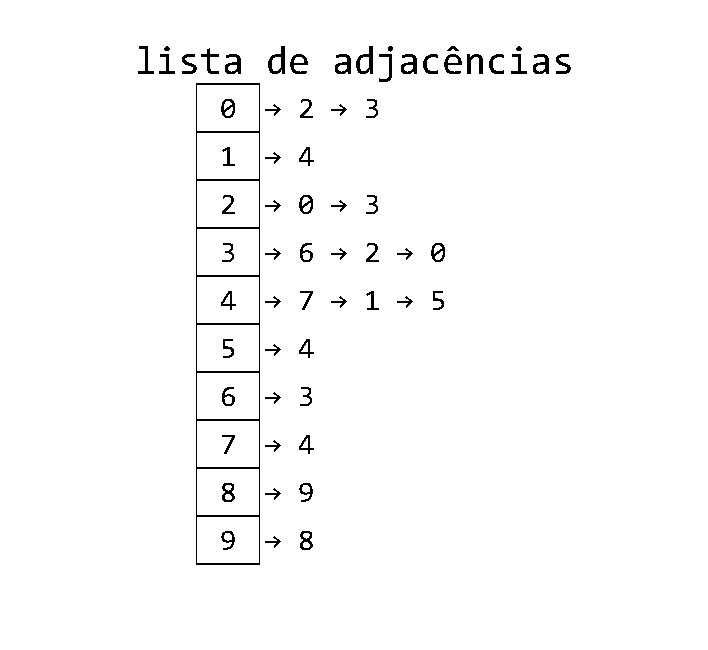
\includegraphics[width=\linewidth]{figB.pdf}
	}
	\subcaptionbox{}[.32\textwidth]
	{
		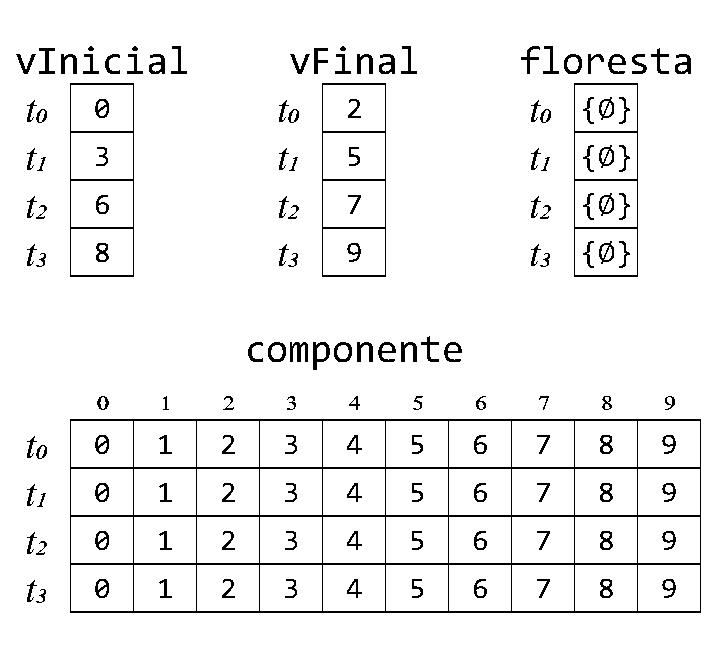
\includegraphics[width=\linewidth]{figC.pdf}
	}
	\subcaptionbox{}[.32\textwidth]
	{
		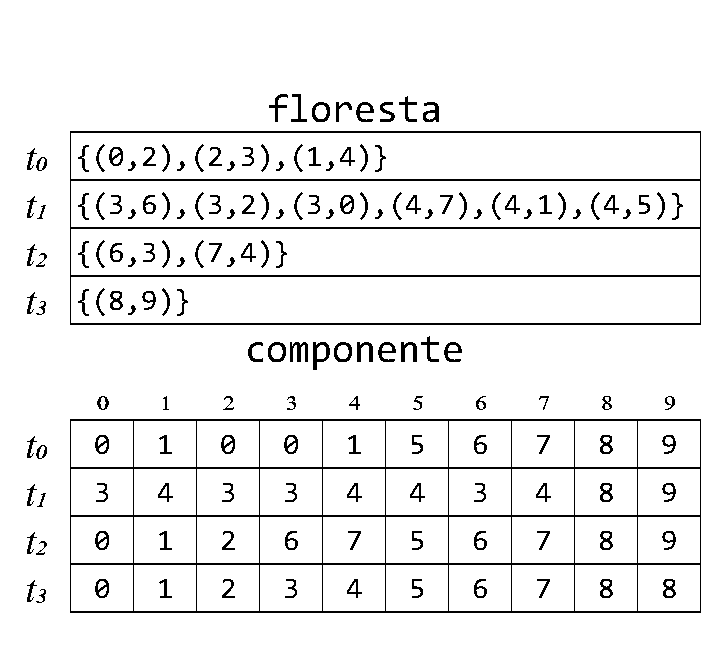
\includegraphics[width=\linewidth]{figD.pdf}
	}
	\subcaptionbox{}[.32\textwidth]
	{
		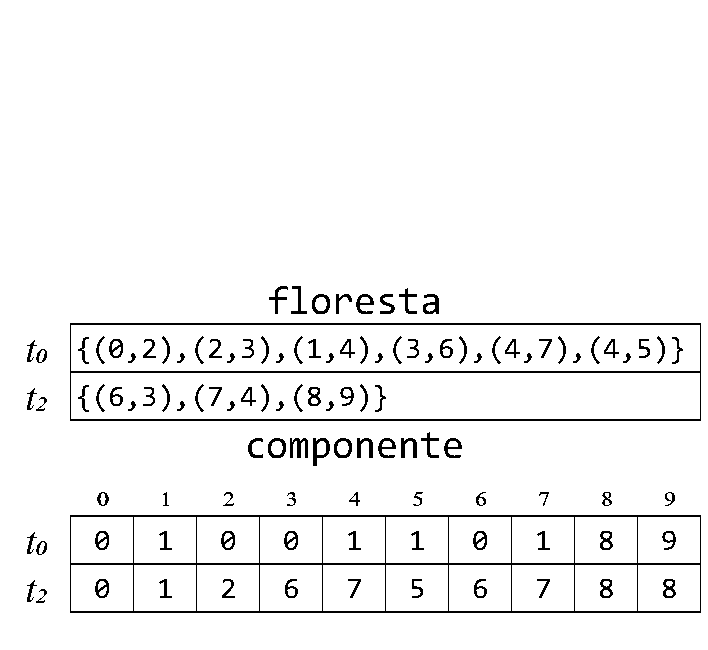
\includegraphics[width=\linewidth]{figE.pdf}
	}
	\subcaptionbox{}[.32\textwidth]
	{
		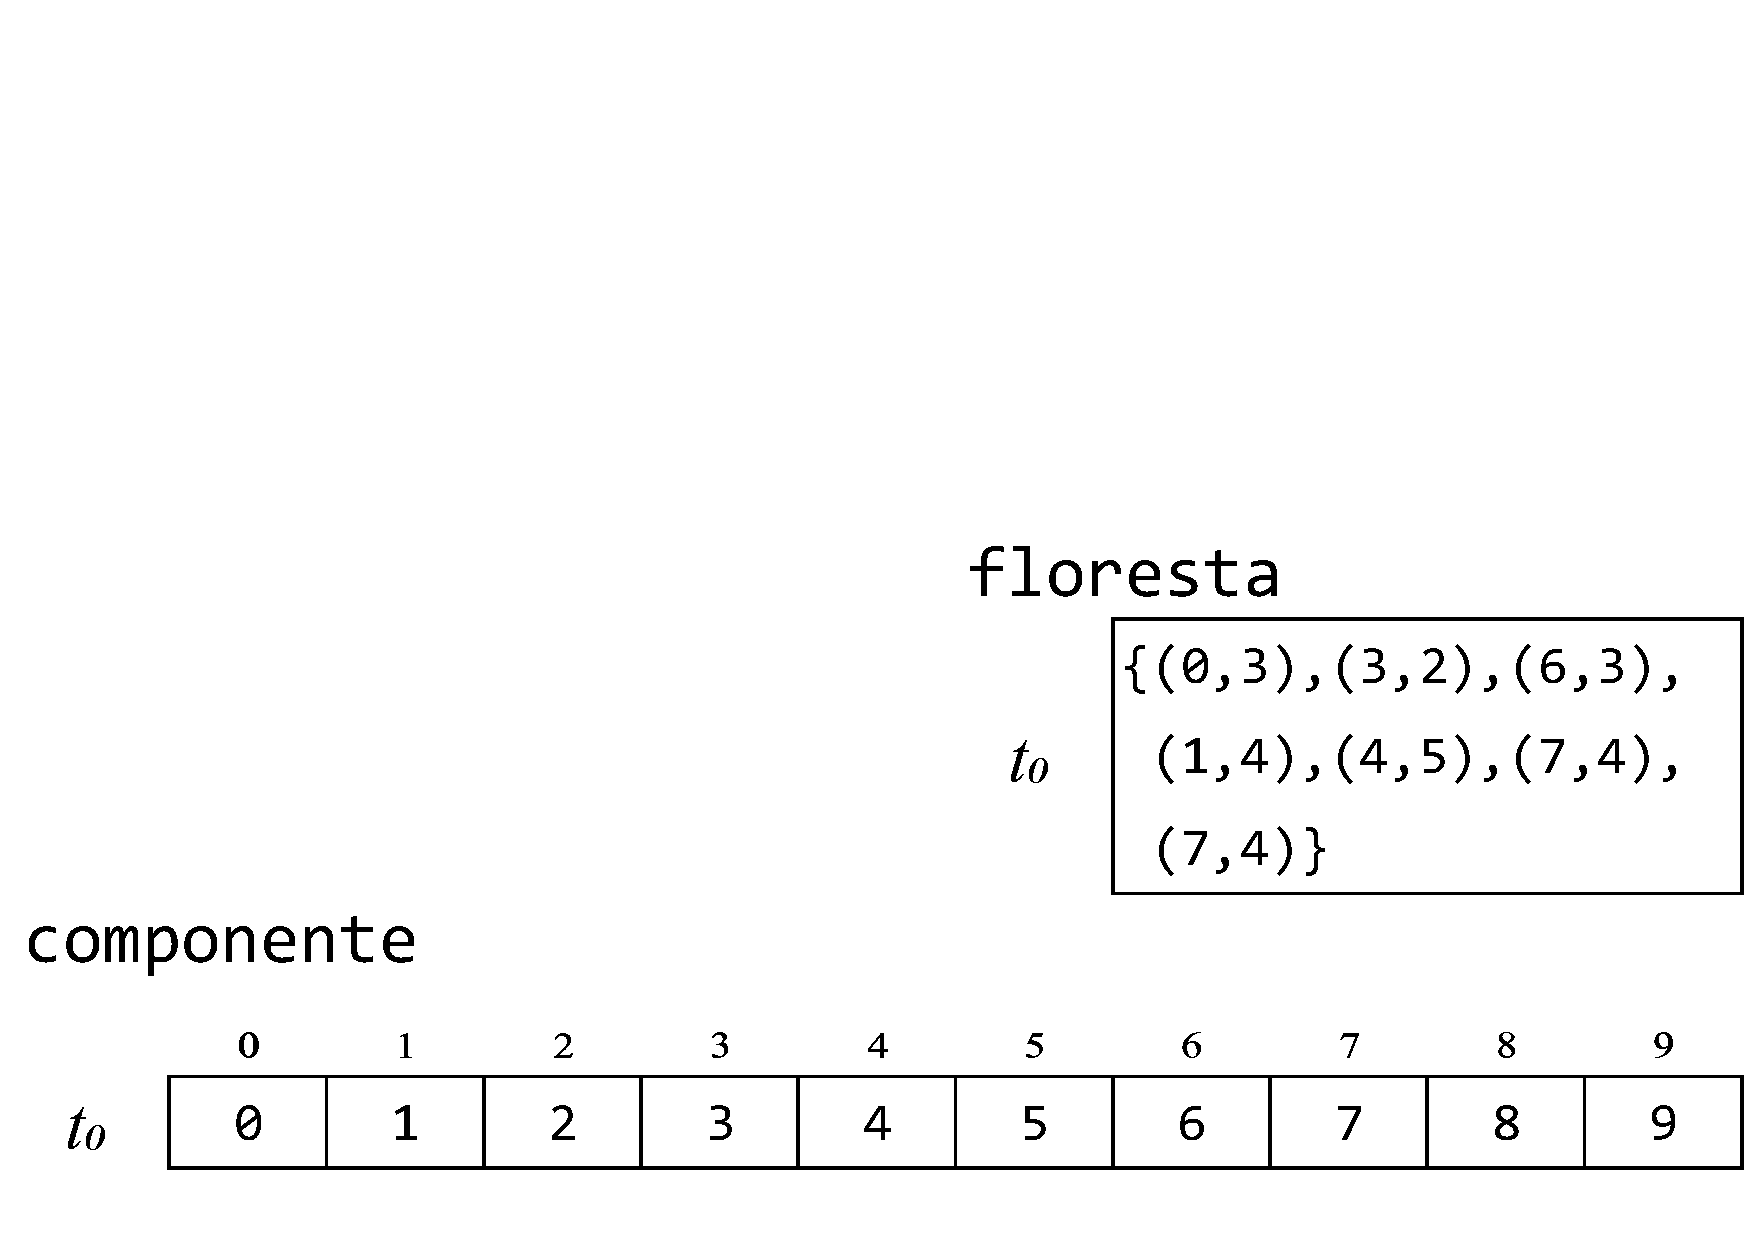
\includegraphics[width=\linewidth]{figF.pdf}
	}
	\caption{Ilustração dos passos da execução do algoritmo paralelo. (a) Representação gráfica de G=(V, E). (b) Lista de adjacências do grafo G. (c) Estado das estruturas antes de iniciar a busca em profundidade paralela. (d) Estado das estruturas após terminar a busca em profundidade paralela. (e) Estado das estruturas após fazer a primeira rodada de uniões em paralelo. (f) Estado das estruturas após fazer a segunda rodada de uniões. Note que, a thread 0 possui o resultado do algoritmo.}
		\label{fig:1}
\end{figure}

\newpage
\section{Resultados e Análise}

Para mensurar o desempenho dos dois algoritmos implementados, foi utilizado como entrada, um grafo gerado aleatoriamente. A fim de observar o comportamento dos algoritmos em diferentes tipos de grafos, dividimos os mesmos em relação a tamanho (quantidade de vértices) e densidade (quantidade de arestas em relação à quantidade máxima de arestas possíveis do grafo).

Os tamanhos escolhidos foram: 5~000, 10~000, 15~000 e 25~000 vértices. Apesar de os tamanhos serem aparentemente pequenos, a busca em profundidade analisa todas as arestas do grafo e não somente os vértices, logo, para um grafo k-completo de 25~000 vértices, teremos 312~487~500 arestas. As densidades escolhidas foram: 10\%, 25\%, 50\%, 75\% e 100\%. Um grafo de densidade 10\% possui, independentemente do número de vértices, 10\% de arestas da quantidade máxima de arestas que pode possuir. Um grafo de densidade 100\% é simplesmente um grafo k-completo. Para ilustrar as variações entre tamanho e densidade, temos como exemplo que um grafo de 5~000 vértices e densidade de 25\%, irá possuir 3~124~375 arestas.

A máquina onde os testes foram executados encontra-se na FACOM, sendo ela um Dell Precision, processador Intel Xeon E5-1620 v3 3.5GHz, 4 núcleos, 8 threads e 32 GB de RAM. O compilador utilizado foi o GCC versão 7.4 (com a opção -O3) e o sistema operacional utilizado foi o Ubuntu 16.04 x86\_64. Os dados obtidos nos testes foram compilados a partir de 5 execuções de cada algoritmo, para cada tamanho e densidade do grafo de entrada.

As Figuras~\ref{fig:2} e \ref{fig:3} ilustram graficamente os tempos de execuções dos algoritmos, dado as diferentes entradas. Na figura~\ref{fig:2} a densidade do grafo de entrada é fixada em 100\% e na Figura~\ref{fig:3} o tamanho do grafo de entrada é fixado em 25~000 vértices. Em ambas as figuras são comparados os tempos de execução do algoritmo sequencial e do paralelo com 16 \emph{threads}. É possível notar que, o tempo de execução do algoritmo sequencial aumenta exponencialmente quando se varia a quantidade de vértices sendo que, no algoritmo paralelo, apesar de não ser linear, o aumento do tempo de execução é bem menor. Também se nota que a densidade do grafo de entrada impacta muito mais o tempo de execução do algoritmo sequencial do que o tempo do algoritmo paralelo.

\begin{figure}[H]
    \centering
    \begin{minipage}{.48\textwidth}
        \centering
        \resizebox{\textwidth}{!}
        {
			\begin{tikzpicture}
			\begin{axis}[
				%title={Execução alg par 25k com várias threads},
				legend pos=north west,
				xlabel={quantidade de vértices},
				%legend style={at={(0.5,-0.20)},anchor=north,legend columns=-1},
				%symbolic x coords={a,b,c,d},
				ylabel={tempo de execução (s)},
				xtick=data,
				symbolic x coords={5K, 10K, 15K, 25K}]
				\addplot coordinates {
					(5K,2.8425)(10K,12.9809)(15K,35.0820)(25K,105.7478)};
				\addplot coordinates {
					(5K,0.9850)(10K,4.2318)(15K,10.5094)(25K,30.9745)};
			\legend{Sequencial, Paralelo}
			\end{axis}
			\end{tikzpicture}
		}
        \caption{Tempo de execução, densidade fixada em 100\% e paralelo com 16 \emph{threads}}
        \label{fig:2}
    \end{minipage}\hfill%
    \begin{minipage}{.48\textwidth}
        \centering
        \resizebox{\textwidth}{!}
        {
			\begin{tikzpicture}
			\begin{axis}[
				%title={Execução alg par 25k com várias threads},
				legend pos=north west,
				xlabel={densidade do grafo},
				%legend style={at={(0.5,-0.20)},anchor=north,legend columns=-1},
				%symbolic x coords={a,b,c,d},
				ylabel={tempo de execução (s)},
				xtick=data,
				symbolic x coords={5\%, 25\%, 50\%, 75\%, 100\%}]
				\addplot coordinates {
					(5\%,3.7357)(25\%,22.9317)(50\%,50.8209)(75\%,77.6357)(100\%,105.7478)};
				\addplot coordinates {
					(5\%,1.3433)(25\%,8.1235)(50\%,16.6858)(75\%,24.3761)(100\%,30.9745)};
			\legend{Sequencial, Paralelo}
			\end{axis}
			\end{tikzpicture}
		}
        \caption{Tempo de execução, tamanho fixado em 25K e paralelo com 16 \emph{threads}}
        \label{fig:3}
    \end{minipage}
\end{figure}

As Figuras~\ref{fig:4} e \ref{fig:5} ilustram graficamente o \emph{speedup} alcançado pelo algoritmo paralelo em relação ao algoritmo sequencial. Nas duas figuras temos todas as entradas analisadas no teste, variando o eixo de exibição. É interessante notar que há uma variação de desempenho no grafo de entrada de 10~000 vértices, já  que ele não segue o “padrão” visto nos outros grafos de entrada. Inicialmente, pensou-se que isso se devia a um caso isolado, mas após várias execuções, esse desempenho se repetiu. Também se nota que o algoritmo paralelo, com o maior e mais denso grafo de entrada, foi 3.4 vezes mais rápido que o algoritmo sequencial.

\begin{figure}[H]
    \centering
    \begin{minipage}{.48\textwidth}
        \centering
        \resizebox{\textwidth}{!}
        {
			\begin{tikzpicture}
			\begin{axis}[
				%title={Execução alg par 25k com várias threads},
				legend style={at={(0.5,1.15)},anchor=north,legend columns=-1},
				xlabel={quantidade de vértices},
				%legend style={at={(0.5,-0.20)},anchor=north,legend columns=-1},
				%symbolic x coords={a,b,c,d},
				ylabel={\emph{speedup}},
				xtick=data,
				symbolic x coords={5K, 10K, 15K, 25K}]
				\addplot coordinates {
					(5K,2.0066)(10K,2.5546)(15K,2.5800)(25K,2.7810)};
				\addplot coordinates {
					(5K,2.7384)(10K,2.7336)(15K,2.6243)(25K,2.8229)};
				\addplot coordinates {
					(5K,2.6475)(10K,2.7354)(15K,2.7931)(25K,3.0458)};
				\addplot coordinates {
					(5K,2.7349)(10K,2.8928)(15K,3.0592)(25K,3.1849)};
				\addplot coordinates {
					(5K,2.8858)(10K,3.0675)(15K,3.3382)(25K,3.4140)};
			\legend{5\%, 25\%, 50\%, 75\%, 100\%}
			\end{axis}
			\end{tikzpicture}
		}
        \caption{\emph{Speedup} paralelo em relação ao sequencial, paralelo com 16 \emph{threads}}
        \label{fig:4}
    \end{minipage}\hfill%
    \begin{minipage}{.48\textwidth}
        \centering
        \resizebox{\textwidth}{!}
        {
			\begin{tikzpicture}
			\begin{axis}[
				legend pos=north west,
				%legend style={at={(0.5,1.15)},anchor=north,legend columns=-1},
				%xlabel={densidade do grafo},
				%legend style={at={(0.5,-0.20)},anchor=north,legend columns=-1},
				%symbolic x coords={a,b,c,d},
				ylabel={\emph{speedup}},
				xlabel={densidade do grafo},
				xtick=data,
				symbolic x coords={5\%, 25\%, 50\%, 75\%, 100\%}]
				\addplot coordinates {
					(5\%,2.0066)(25\%,2.7384)(50\%,2.6475)(75\%,2.7349)(100\%,2.8858)};
				\addplot coordinates {
					(5\%,2.5546)(25\%,2.7336)(50\%,2.7354)(75\%,2.8928)(100\%,3.0675)};
				\addplot coordinates {
					(5\%,2.5800)(25\%,2.6243)(50\%,2.7931)(75\%,3.0592)(100\%,3.3382)};
				\addplot coordinates {
					(5\%,2.7810)(25\%,2.8229)(50\%,3.0458)(75\%,3.1849)(100\%,3.4140)};
			\legend{5K, 10K, 15K, 25K}
			\end{axis}
			\end{tikzpicture}
		}
        \label{fig4}
        \caption{\emph{Speedup} paralelo em relação ao sequencial, paralelo com 16 \emph{threads}}
        \label{fig:5}
    \end{minipage}
\end{figure}

Por padrão, o OpenMP utiliza a quantidade de \emph{threads} disponíveis do processador. A fim de executar mais testes, forçamos quantidades diferentes de threads para analisar o comportamento do algoritmo paralelo. Como é visto nas Figuras~\ref{fig:6} e \ref{fig:7}, o melhor resultado em tempo de execução foi ao utilizar 16 \emph{threads}. Apesar de não haver diferença expressiva entre o uso de 8 ou 16 \emph{threads}, optou-se por utilizar a execução de 16 \emph{threads} para analisar o desempenho do algoritmo paralelo, pois, nela foi obtido o melhor desempenho.

\begin{figure}[!htp]
    \centering
    \begin{minipage}{.48\textwidth}
        \centering
        \resizebox{\textwidth}{!}
        {
			\begin{tikzpicture}
			\begin{axis}[
				legend pos=north west,
				xlabel={quantidade de vértices},
				%legend style={at={(0.5,-0.20)},anchor=north,legend columns=-1},
				%symbolic x coords={a,b,c,d},
				ylabel={tempo de execução (s)},
				xtick=data,
				symbolic x coords={5K, 10K, 15K, 25K}]
				\addplot coordinates {
					(5K,2.0038)(10K,8.4621)(15K,21.8479)(25K,64.3706)};
				\addplot coordinates {
					(5K,1.2820)(10K,5.8591)(15K,14.8007)(25K,41.4975)};
				\addplot coordinates {
					(5K,1.0018)(10K,4.3181)(15K,10.5758)(25K,31.0767)};
				\addplot coordinates {
					(5K,0.9850)(10K,4.2318)(15K,10.5094)(25K,30.9745)};
			\legend{2 $th$,4 $th$,8 $th$, 16 $th$}
			\end{axis}
			\end{tikzpicture}
		}
        \caption{Tempo de execução do algoritmo paralelo, densidade fixada em 100\%}
        \label{fig:6}
    \end{minipage}\hfill%
    \begin{minipage}{.48\textwidth}
        \centering
        \resizebox{\textwidth}{!}
        {
			\begin{tikzpicture}
			\begin{axis}[
				legend pos=north west,
				xlabel={densidade do grafo},
				%legend style={at={(0.5,-0.20)},anchor=north,legend columns=-1},
				%symbolic x coords={a,b,c,d},
				ylabel={tempo de execução (s)},
				%xtick=data,
				symbolic x coords={5\%, 25\%, 50\%, 75\%, 100\%}]
				\addplot coordinates {
					(5\%,2.4396)(25\%,15.6663)(50\%,33.4889)(75\%,51.2299)(100\%,64.3706)
				};
				\addplot coordinates {
					(5\%,1.6939)(25\%,11.2393)(50\%,22.2700)(75\%,35.0567)(100\%,41.4975)
				};
				\addplot coordinates {
					(5\%,1.3561)(25\%,8.1547)(50\%,16.7268)(75\%,24.5019)(100\%,31.0767)
				};
				\addplot coordinates {
					(5\%,1.3433)(25\%,8.1235)(50\%,16.6858)(75\%,24.3761)(100\%,30.9745)
				};
			\legend{2 $th$,4 $th$,8 $th$, 16 $th$}
			\end{axis}
			\end{tikzpicture}
		}
        \caption{Tempo de execução do algoritmo paralelo, tamanho fixado em 25K}
        \label{fig:7}
    \end{minipage}
\end{figure}

\section{Conclusão}

A descrição do algoritmo paralelo visto em~\cite{Grama:2003} é muito alto nível para a união das florestas. Implementar este algoritmo mostrou-se ser desafiador para o autor deste trabalho. Os detalhes das estruturas e a maneira como foi implementada a união das florestas, foi concebida do zero, sem ter referências para se apoiar. Em contrapartida, utilizar a interface de programação OpenMP, facilitou e muito a implementação do paralelismo no algoritmo. Não houve teste com tamanhos maiores de grafos, pois, o tamanho ocupado fisicamente pelo grafo de entrada é muito grande, sendo que, nos testes que utilizamos tamanhos muito grandes, houve estouro de memória e não foi possível realizar o teste.
\newpage
Como visto no capítulo 4, o algoritmo paralelo teve um ganho de até 3.4 vezes em relação ao sequencial. Ao analisar que o processador testado só possui 4 núcleos, esse ganho se apresenta ser muito satisfatório. Mesmo no pior cenário, o algoritmo paralelo alcançou pelo menos 2 vezes o desempenho do algoritmo sequencial. Apesar das complexidades maiores que o algoritmo paralelo traz em relação ao sequencial (que é relativamente simples e muito bem conhecido na literatura), o desempenho adquirido faz valer toda a dificuldade e põe o algoritmo paralelo como uma boa escolha para resolver o problema dos componentes conexos.

Para trabalhos futuros, é possível melhorar ainda mais a implementação do algoritmo paralelo. As operações \emph{Union-Find} utilizadas na implementação são as mais simples da literatura. Em~\cite{Sedgewick:2011} é apresentado uma versão mais eficiente do \emph{Union-Find}, com pesos e compressão de caminhos, porém, de maior complexidade de implementação. Outra situação vista no algoritmo paralelo aqui implementado se dá ao executar uma rodada de uniões par a par, quando metade das \emph{threads} não serão mais utilizadas na próxima rodada. Analisar e implementar uma maneira de utilizar novamente essas \emph{threads}, poderia trazer um ganho ainda maior para o algoritmo paralelo.

%\newpage
\bibliographystyle{sbc}
\bibliography{sbc-template}

\end{document}
